\documentclass[12pt]{article} % Default font size is 12pt, it can be changed here

\usepackage{graphicx} % Required for including pictures
%\usepackage{float} % Allows putting an [H] in \begin{figure} to specify the exact location of the figure
%\usepackage{floatrow}
\usepackage{wrapfig} % Allows in-line images such as the example fish picture
\usepackage[margin=1in, paperwidth=8.5in, paperheight=11in]{geometry}

\setcounter{tocdepth}{5} %to make it appears in TOC
\setcounter{secnumdepth}{5} %to make it numbered

\linespread{1.2} % Line spacing

\setlength\parindent{0pt} % Uncomment to remove all indentation from paragraphs

\graphicspath{{./Pictures/}} % Specifies the directory where pictures are stored

\date{}

\begin{document}

\title{Not Nyout}
\maketitle

\section{Introduction}

What started as a friendly Nyout race has turned ugly after RED called BLUE's mother fat - now it's a fight to the death!  You must use your horses to eliminate those of each other player and be the last one standing.

\section{Pieces}

\begin{itemize}
	\item 1x Nyout Board
	\item 4x red horses
	\item 4x blue horses
	\item 4x green horses
	\item 4x white horses
	\item 1x 4-sided die
	\item 1x 6-sided die
	\item 1x 8-sided die
	\item 1x 10-sided die
\end{itemize}

\section{Starting the Game}

\subsection{}
Two, three or four players can play.

\subsection{}
Each player picks a color - red, blue, green or white. She starts off with the four corresponding horses \textbf{off of the board} in her stable. \newline

The rest of the set-up is different when there are three or four players than when there are two.

\subsection{With Two Players}

\subsubsection{}
Each player gets one of the cardinal direction square as a home square.  They must be opposite from each other (either N and S or E and W).  

\subsubsection{}
Each players rolls the 10-sided die to decide who starts.  The player with the highest roll starts first.  If there is a tie each player rerolls.

\subsection{With Three or Four Players}

\subsubsection{}
Each player rolls the 10-sided die.  Ties are broken by rerolling.  Then each player, starting with the player who rolled highest and then going down in order, chooses his turn order for the game.  Therefore, the player who rolled highest could choose to go last, or any of first, second, third or fourth.  Each successive player must pick from the remaining turn slots.

\subsubsection{}
On the each player's first turn of the game, he must pick his home square.  He may pick it after making his first roll.  Two players may not have the same home square.  Therefore in a four player game, the last player to go is forced onto the remaining square.  Immediately after choosing his home square, he summons his first horse onto the board.


\section{A Turn}

\subsection{}
At the beginning of each player's turn, he determines movement by rolling the four-sided die once for each horse group he controls, noting each roll of the die.  If he controls no horses, he rolls once. (For example on the first turn of the game.)  Single horses are considered horse groups of size one.

\subsection{}
All dice rolls for a turn are performed consecutively at the beginning of the turn before any movement is done.

\subsection{}
For each roll, the player may move a horse group that many squares, or summon a new horse onto the board.  \textbf{All of the rolls must be used}.

\subsection{Summoning Horses}

\subsubsection{}
Once per turn, if a player has any horses left in her stable, she may use one of her rolls to summon a new horse onto the board.  

\subsubsection{}
The horse starts counterclockwise of her home square the number of squares equivalent to the roll of the die used to summon the horse.  Each square around the outer circle is labeled to indicate the player and die roll to summon a horse there.  For example, if the player who's home square is "S" uses a roll of 3 to summon a horse, it would enter the board on the square labeled "S3".

\subsubsection{}
Horses may be summoned onto an occupied square.   If the square is occupied by another of the player's horses, the may be joined immediately.  If the square is occupied by an opposing player's horse, it initiates combat immediately.  (More on each of those later.)

\subsubsection{}
Additional die rolls may be used to move a horse on the same turn that it was summoned.

\subsection{Moving Horses}

\subsubsection{}
The dice throws may be used to move horses a number of squares equivalent to the number shown on the die.  

\subsubsection{}
Multiple die rolls may be used on a single horse.  But each die roll is conducted as a separate movement.  If a roll of three and a roll of four are used on the same horse, it either moves three squares then four, or four then three.  

\subsubsection{}
 Horses always move around the outer ring of squares in a counterclockwise direction.

\subsubsection{}
If a horse is sitting on one of the cardinal directions - N, S, E or W - before it starts moving, it may move onto the center squares.  \textbf{A horse cannot turn towards the center in the middle of a movement}.

\subsubsection{}
While on either the vertical column, or horizontal row of squares that goes through the middle of the board, a horse group may be moved either towards or away from the center. When passing the center square in the middle of a movement, a horse may continue straight or turn in any direction but it may not turn backwards in the same direction it came from.  When reentering the outer circle from one of the cardinal squares, it must turn to move counterclockwise.\newline

\newpage

For example, in the following diagram, if a horse group starts at S, a roll of 3 would get it to any of the squares marked E.  It could not get to X1 by moving towards the center and then moving backwards.  Nor could it get to X2 by moving down and then turning clockwise.\newline

\centerline{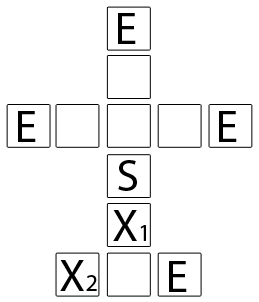
\includegraphics[scale=.75]{notnyoutdiagram1.png}}

\subsubsection{}
If a horse must pass an enemy horse, an additional movement is used.  For instance, to move 2 squares, with an enemy in the way, it would take a roll of 3.\newline

For example, in this diagram, if R represents a red horse group and B a blue horse group, the red player would need to roll a 1 to get the horse group to the square marked 1, but it would need a 4 to get to the square marked 4.  Both 2 and 3 would make the horse group land on the same square as blue.\newline

\centerline{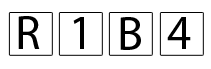
\includegraphics[scale=1]{notnyoutdiagram2.png}}

\subsection{Joining Horses}

\subsubsection{}
Immediately after a player's horse groups lands on the same square as another of his horse groups, they may be joined into one group.  \textbf{Joining horses is optional}. 

\subsubsection{}
A group can have up to four horses joined together.

\subsubsection{}
Horses groups may be separated on a player's turn, after the movement dice have been rolled.  Therefore, if a player has two horse groups at the beginning of his turn, and rolls two movement dice, he doesn't get an additional die roll that turn by splitting one of his groups after.  

\subsubsection{}
A group may be separated in any way.  For example, a group of four may be seperated into four groups of one, a group of two and two groups of one, two groups of two, or a group of three and a group of one.


\subsection{Combat}

\subsubsection{}
If a player's horse lands on the square as an enemy's horse, it initiates combat.  

\subsubsection{}
Combat is determined by dice rolls.  The die rolled by each player is determined by the number of horses in his group:
\begin{itemize}
	\item 1 horse:  4-sided die
	\item 2 horses: 6-sided die
	\item 3 horses: 8-sided die
	\item 4 horses: 10-sided die	
\end{itemize}

\subsubsection{}
The player who initiated combat gets a +2 bonus added to his die roll.

\subsubsection{}
The winner is the player with the higher total number.  If it is a tie, the victory goes to the player who didn't initiate combat.  The loser loses one horse from the horse group that was in combat.\newline

 For example, if blue moves a group with two horses onto a square where red has a group with three horses, blue will roll a 6-sided die and add 2 to his die roll, while red will roll an 8-sided die.  If the two totals are equal, then red is the winner.

\section{Ending the Game}

\subsection{}
The game ends when only a single player has any horses left on the board.

\subsection{}
Alternatively, if the game is down to two players, each with a single horse, then five full rounds after the last horse was taken the game ends, and the last player to kill a horse is declared the winner.  \newline

For example, if the game was down to red with one horse and blue with two horses, and red killed one of blue's horses, then neither player killed each other in the following five rounds, red is the winner.


\end{document}